\chaptertitle{10}{四种定投方法，哪种更适合你}


\setcounter{figure}{0}\setcounter{table}{0}
在前面的章节中，我们了解了提高定投收益有如下技巧。

\begin{itemize}
\item 选择长期收益优秀的策略加权指数基金和优秀行业指数基金。
\item 在熊市指数基金处于低估的阶段定投。
\end{itemize}

不过具体在定投的时候，还有一个问题：买多少？

通常我们接触的定投，都是定期定额定投的，那定投究竟是不是必须要定期定额呢？

\subsection{定期定额的定投，在A股并不适用}
首先说说定期定额的定投方法。

定期定额就是选择一个固定日期，然后投入相同的金额。比如说，在每个月的第一天定投2000元的指数基金。

这就是定期定额的定投方法。也就是说，你每次定投基金的时间和金额是固定不变的。

不过针对A股，不建议大家采用定期定额的定投方法。

{\heiti 中国的人均收入增长较快}

国内公募基金诞生的时间并不长，真正普及也就是最近十几年的事情。

早期国内有关基金的研究也不多，很多基金方面的资料是来自海外市场，特别是来自美国、日本等基金市场。在这些相关书中，介绍定投的操作，通常说的都是定期定额的。

不过在A股，我们就不能用定期定额的方法了。

不同国家的人均收入增速有非常大的差别。中国是一个高速发展中的国家，国内人均可支配收入增速在过去20年，保持了两位数的年复合增长率。这是一个很伟大的奇迹。20世纪90年代的时候，月收入几百元是平均水平，而到了现在，大部分人的月收入是几千元。提升速度非常快。而像日本等成熟市场，人们的月收入已经很长时间没有上涨了。从1998年到2015年，日本人的月收入不仅没有上涨，反而是略微下降的。在日本，同一家公司、同一个岗位的薪水，有可能不如20年前。

假如一个日本上班族做定投的操作，他即便是采用定期定额的定投，都是比较吃力的，因为他的收入可能在慢慢降低。

但是对中国的上班族来说，定期定额定投，是不可行的。比如说20世纪90年代，月收入是1000元，我们拿出200元定投，这就是比较高的了。但是在2019年，大部分人的月收入是数千元。只拿出200元定投，就完全不够。

从这个案例，我们可以看出，定期定额的定投并不一定是适合所有国家的投资者的。不同的国家情况不同，不能直接照搬。

所以在国内，定期定额的定投，只能是一个短期的设置。时间稍长一些，就需要提高定投的金额，因为人均收入增长较快。每隔几年，就需要根据家庭收入的增长速度，重新按比例决定定投的金额。

{\heiti 相同金额的购买力随时间在下降}

我们来看这样一个案例，如果我们从2015年开始，每个月拿出1000元定投，持续10年，会发生什么呢？

10年后，我们会持有几十万元市值的指数基金，但是仍然是每个月买入1000元。实际上因为通货膨胀、指数上涨等原因，10年后的1000元能买到的指数基金份额，只是现在的一小部分。换句话说，如果我们定投的金额不变，实际上买入的基金份额在逐渐减少。

这就是定额定投的最大缺点：相同金额的购买力随时间在下降。

既然定期定额有缺陷，那有没有其他的方式来决定定投的金额，从而获得更好的收益呢？

这就是接下来螺丝钉要跟大家介绍的定投方法：定期不定额。

\subsection{定期不定额，收益才更好}
{\heiti 定期不定额的定投方法}

除了收入的原因之外，指数基金自己的涨跌，也会导致投资价值的变化。

我们前面介绍过，指数基金可以长期上涨。

特别是我们投资的优秀宽基指数基金和优秀行业指数基金，长期涨幅都是不错的。我们在低估区域定投这些指数基金，如果短期内指数基金下跌了，它的投资价值实际上是提高的。

在短期的时间里，指数基金处于不同估值，其投资价值也会有很大的差别。我们一直在说，要在指数基金低估的时候才去投资。可能指数基金短短一年时间里就会有上下30\%的波动，可能会出现高估值，也可能会出现低估值，我们自然要在指数基金处于低估值的时候定投更多的资金，这样才能获得更好的收益。

这就是定期不定额定投的来源，我把这个提升收益的技巧叫作“定投收益放大器”。

{\heiti 在“微笑曲线”的左侧买入，越跌越买}

如图 \ref{fig:10-1} 所示，在“微笑曲线”的左侧，是下跌，到了右侧是上涨。

通常我们定投是从进入低估开始的，也就是从左侧开始定投。在“微笑曲线”的左侧越跌越买，到了右侧不需要涨到原来位置就能开始赢利，如果能涨到原来位置，那收益会更好。

\begin{figure}[htbp]
\centering
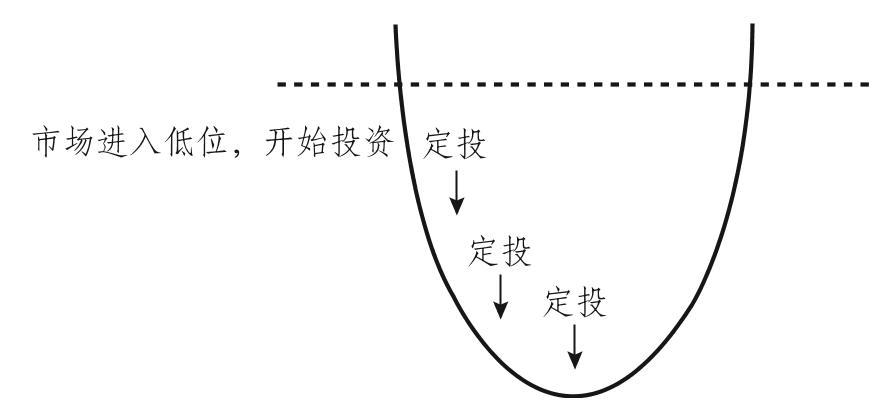
\includegraphics[width=\textwidth,height=0.82\textheight,keepaspectratio]{figure/图10.1.png}
\caption{在“微笑曲线”左侧定期定额定投}\label{fig:10-1}
\end{figure}

在这个基础上，因为指数基金上涨是长期的，下跌是短期的。如果我们在下跌的过程中，适当提高定投的金额，如图 \ref{fig:10-2} 所示，那“微笑曲线”的作用还会更强，从而进一步提高收益，也就是“越跌越买”的思路。

\begin{figure}[htbp]
\centering
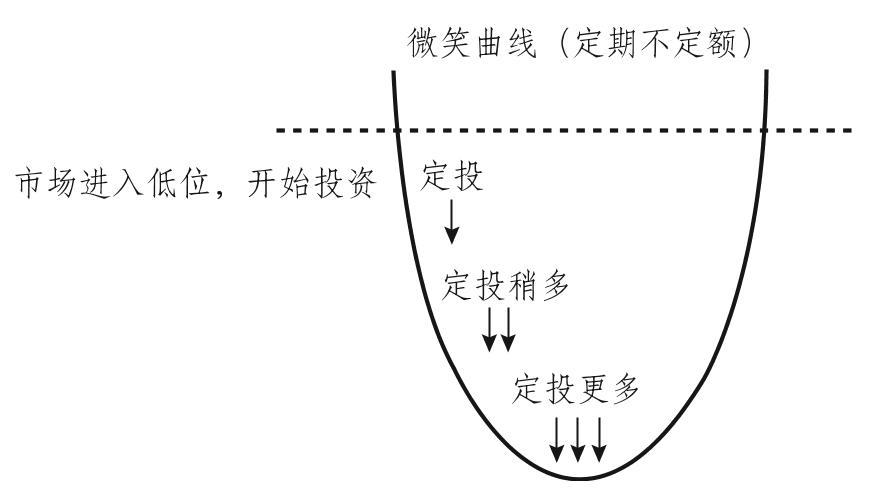
\includegraphics[width=\textwidth,height=0.82\textheight,keepaspectratio]{figure/图10.2.png}
\caption{在“微笑曲线”左侧定期不定额定投}\label{fig:10-2}
\end{figure}

定期不定额定投有很多种，不过核心的思路都是：越下跌，定投市场进入低位，开的始时投候资买定入投越多。

这里介绍三种采用“越跌越买”思路的定投方法。

第一种是慧定投，基于均线的定期不定额定投方法。

第二种是价值平均策略，基于市值的定期不定额定投方法。

第三种是估值定投策略，基于估值的定期不定额的定投方法。

\subsection{慧定投：基于均线的定期不定额}
{\heiti 什么是慧定投}

第一种方法叫作慧定投。

如果有用支付宝来投资指数基金的朋友，可能会看到，在定投的时候，会有一个慧定投的选项。

这个慧定投是什么呢？

慧定投就是定期不定额的一种投资方式，它参考的是均线。

均线是股票投资经常用到的一个参考数据。所谓的均线，就是用过去一段时间的平均价格绘制出的曲线。

比如说支付宝的慧定投，可以选择用500日均线。这里的500日均线，就是最近500个交易日的平均价格。

如果当前的价格高于过去500个交易日的平均价格，那定投的时候就会少投一些。并且高的幅度越大，定投的金额也会减少得更多。

如果当前的价格低于过去500个交易日的平均价格，那定投的时候就会多投一些。并且低的幅度越大，定投的金额也会增加得更多。

参考的均线期限越长，均线本身的变化会更缓和一些。理论上参考长期均线做慧定投，会更可靠一些。

慧定投的规则也不是一成不变的，不过大致的原理就是这样。大家可以在支付宝查看最新的说明。

因为在大涨后减少了定投金额，在下跌后增加了定投金额，慧定投本身是有效果的。

{\heiti 慧定投的两个不足之处}

慧定投的第一个缺陷，是适合的品种有限。

我们前面介绍过，A股有数百只指数基金，很多指数基金追踪的指数是有差别的。它们并不是同涨同跌，长期下来收益也会有区别。

按照慧定投的原理，在定投每一只指数基金的时候，应该参考其对应指数的均线。

比如说投资沪深300指数基金时，参考沪深300指数的均线；投资基本面50指数基金时，参考基本面50指数的均线。

不过截至2019年5月，支付宝的慧定投，只能参考沪深300、中证500、创业板这三个主要宽基指数的历史数据。

比如说我们要投资基本面50或者中证消费行业指数基金，它们的走势跟沪深300指数并不是完全匹配的，所以慧定投就会有缺陷。

目前支付宝的慧定投，最适合的就是沪深300、中证500，以及创业板这三个指数对应的指数基金。

这个缺陷并不难解决，后续如果支付宝了解更多的细分指数基金品种，增加对应指数的历史数据和均线选择即可。

慧定投的第二个缺陷，是无法解决投什么基金收益更好的问题。

按照支付宝的设定，任何一只指数基金都可以用慧定投来投资。不过我们前面也介绍过，不同的指数基金，长期收益有很大差别。长期收益更好的宽基指数基金和优秀行业指数基金，定投下来收益更高。

所以还是需要先选好品种，再做慧定投。慧定投本身无法帮助投资者识别该投资什么的问题。

不过总体来说，慧定投与定期定额的定投相比，还是可以提高收益的。

如果在支付宝定投沪深300、中证500、创业板的指数基金，不妨考虑用慧定投的方式。

\subsection{价值平均策略：基于市值的定期不定额}
{\heiti 什么叫价值平均策略}

第二种方法是价值平均策略。

价值平均策略是20世纪90年代在美国兴起的一种定投方法。有的时候它也被称为市值恒定策略。

简单来说，价值平均策略，就是给手里的指数基金设定一个市值增长速度。

比如说，设定的目标是：保证让手里的指数基金市值，每个月增长1000元。

{\kaishu 第一个月，我们买入1000元的指数基金。}

{\kaishu 第二个月，我们打开账户，发现市场出现了下跌，我们第一个月买入的指数基金，现在只有950元了。按照计划，我们第二个月，需要持有2000元的指数基金。所以第二个月，我们就不能定投1000元，而是需要定投1050元。这样第二个月投完，我们就持有2000元市值的指数基金。}

{\kaishu 第三个月，我们的目标是3000元。但是打开账户，发现指数基金上涨了，我们持有2100元的指数基金。这样第三个月就只需要定投900元。}

这就是价值平均策略，也被称为市值恒定策略。

这个金额增长速度，可以设定为每个月增加多少元，也可以设定为每个月增加百分之多少。

这种定投方法，非常适合为某个目标积累财富。比如说10年后我们要200万元来买房，那就可以设定一个价值平均策略的定投方案，让我们持有的市值一步步按照计划来，到第10年，正好达到200万元的市值。

{\heiti 价值平均策略的缺点}

不过这种策略也有一个缺点：如果遇到股市大跌，需要短期内拿出比较多的资金来补仓。

比如说按照计划，我们已经持有了50万元的指数基金，下个月的目标是51万元。但是遇到了股市短期大跌，指数基金短期下跌了30\%。这种情况并不罕见，每隔几年A股就很有可能遇到一次。那持有的指数基金市值，就变成了35万元。那下个月如果还想达成51万元的目标，就需要一次性拿出16万元。

这可不是一笔小数字。对于波动高的A股来说，这个问题迟早会遇到。

价值平均策略，相比前面介绍的慧定投，对资金量的考验会更大一些。

不过也有解决方法。有的投资者，会对价值平均策略每个月投入金额做一个上限，比如说遇到需要一次性买入很多的时候，最多一个月只投入1万元。有了这个上限，压力就小很多了。

同样地，价值平均策略与定期定额的定投相比，也可以获得更好的长期收益。

从1926年到2006年，如果用定期定额的定投方法，年化收益率大约是10.85\%。而如果用价值平均策略来定投，年化收益率大约是12.39\%。平均每年有1.54\%的超额收益。

同样地，使用价值平均策略，也需要选择长期收益更好的指数基金品种，才能有更好的定投效果。

\subsection{估值定投策略：基于估值的定期不定额}
{\heiti 基于估值的定期不定额}

慧定投和价值平均策略，本身都是有效的。不过这两种定投方式，本身没有考虑指数基金自身的投资价值。

我们前面介绍过，最好在指数基金处于低估的阶段去投资，这样可以获得更好的长期收益。

国内有70\%的投资者，是在牛市股市大涨之后才开始接触指数基金的。如果在牛市估值很高的时候开始定投指数基金，即便是采用慧定投或者价值平均策略，仍然可能在短期内遇到非常大的亏损。

比如说2007年牛市和2015年牛市，之后A股都出现了超过50\%的跌幅。

虽然坚持定投几年，投资者还是可以扭亏为盈。但是有几个人能在50\%的浮亏下还能坚持定投呢？

所以我们可以把定投跟指数基金的估值结合起来。

\begin{itemize}
\item 在熊市指数基金处于低估的阶段开始投资。低估区域，指数基金下跌风险会更小，长期收益也会更理想。
\item 配合估值，对同一只指数基金来说，通常估值越低，投资价值越高，也越值得定投买入更多的金额。
\end{itemize}

这就是基于估值的定期不定额的定投方法，也是螺丝钉一直在长期实践的定投方法。

{\heiti 定投放大器，能够放大我们的投资收益}

举个例子，一只指数基金，适合用盈利收益率来估值。通常对同一个品种，自身盈利收益率上升了，定投价值会越高，定投的时候也就越值得投入更多的资金。则每月定投金额的计算公式为：

\begin{figure}[htbp]
\centering
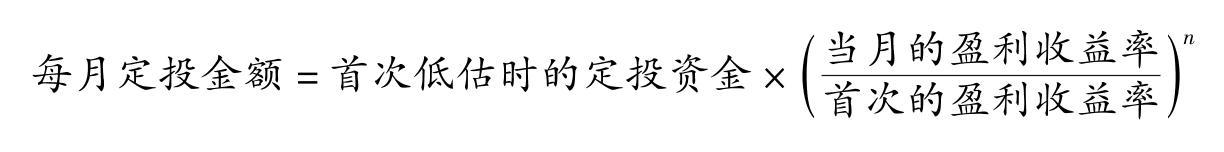
\includegraphics[width=\textwidth,height=0.82\textheight,keepaspectratio]{figure/图10.3.png}
\caption{定投放大器计算公式}\label{fig:10-3}
\end{figure}
在上述公式里有一个\textit{n}，它就是定投收益的放大器，对进一步提升我们定投的收益起着很重要的作用。所谓放大，很好理解，即\textit{n}越大，收益会相对越高。只要普通定期定额的定投是盈利的，那么\textit{n}就能放大我们的收益。

我们以H股指数基金为例来计算一下，这个\textit{n}是如何发挥作用的。

首先，当\textit{n} =0时，0次方都等于1，所以，这时每个月投入的资金都是1000元，固定不变，可以将之看作定期定额定投的收益。假如从2016年的1月开始，每个月都持续定投1000元到H股ETF这只指数基金上（这里1000元是模拟计算的，实际上投资这种场内ETF基金时是按股份数来交易的，并且只能以100股的整数倍来交易）。到2016年11月，一共投入的本金是11000元，持有市值是12123元，可以获得大约10.21\%的投资收益率。

再来看看，假如我们采用定期不定额的方式，在低估的时候买入更多，会发生什么呢？不同的n的取值对我们的投资收益又有什么影响呢？

当\textit{n} =1时，当月的定投金额可以计算如下。

按照计算出的金额来定投，到2016年11月7日，我们共投入的本金是15865元，持有的基金份额是17043份，此时H股ETF的基金净值是1.048元，所以这17043份基金市值是17861元，可以获得约12.58\%的收益率。定期不定额定投比定期定额定投的收益率高了约2\%。

当\textit{n} =2时，当月的定投金额可以计算如下。

按照计算出的金额来定投，到2016年的11月7日，我们共投入的本金是23038元，持有基金的份额是24910份，对应大约26105元的市值，可以获得约13.31\%的收益率，定期不定额定投比定期定额定投的投资收益率，提升了约3\%。具体如表 \ref{tab:10-1} 所示。

{\scriptsize
\setlength{\tabcolsep}{2pt}
\renewcommand{\theHtable}{10-1}
\renewcommand{\arraystretch}{1.2}
\renewcommand{\thetable}{10.1}
\begin{longtable}{>{\centering\arraybackslash}m{0.115\textwidth}>{\centering\arraybackslash}m{0.115\textwidth}>{\centering\arraybackslash}m{0.115\textwidth}>{\centering\arraybackslash}m{0.115\textwidth}>{\centering\arraybackslash}m{0.115\textwidth}>{\centering\arraybackslash}m{0.115\textwidth}>{\centering\arraybackslash}m{0.115\textwidth}>{\centering\arraybackslash}m{0.115\textwidth}}
\caption{2016年1月4日至2016年11月1日，买入份额不同时的投资情况}\label{tab:10-1}\\[1.2ex]
\hline
\noalign{\vskip 4pt}
\bfseries 定投日期 & \shortstack[c]{\bfseries 单位净值\\\bfseries （元）} & \shortstack[c]{\bfseries 盈利收益率\\\bfseries （\%）} & \shortstack[c]{\bfseries 定期定额\\\bfseries 定投（元）} & \shortstack[c]{\bfseries 投入金额\\\bfseries $n=1$（元）} & \shortstack[c]{\bfseries 买入份额\\\bfseries $n=1$（份）} & \shortstack[c]{\bfseries 投入金额\\\bfseries $n=2$（元）} & \shortstack[c]{\bfseries 买入份额\\\bfseries $n=2$（份）} \\
\hline
\endfirsthead
\multicolumn{8}{r}{续表}\\[1ex]
\hline
\noalign{\vskip 4pt}
\bfseries 定投日期 & \shortstack[c]{\bfseries 单位净值\\\bfseries （元）} & \shortstack[c]{\bfseries 盈利收益率\\\bfseries （\%）} & \shortstack[c]{\bfseries 定期定额\\\bfseries 定投（元）} & \shortstack[c]{\bfseries 投入金额\\\bfseries $n=1$（元）} & \shortstack[c]{\bfseries 买入份额\\\bfseries $n=1$（份）} & \shortstack[c]{\bfseries 投入金额\\\bfseries $n=2$（元）} & \shortstack[c]{\bfseries 买入份额\\\bfseries $n=2$（份）} \\
\hline
\endhead
\hline
\endfoot
\hline
\endlastfoot

20161101 & 1.0589 & 12.97 & 1\,000 & 1\,297 & 1\,225 & 1\,682 & 1\,589 \\
20161011 & 1.0596 & 12.84 & 1\,000 & 1\,284 & 1\,212 & 1\,649 & 1\,556 \\
20160901 & 1.0335 & 13.21 & 1\,000 & 1\,321 & 1\,278 & 1\,745 & 1\,688 \\
20160801 & 0.9772 & 13.89 & 1\,000 & 1\,389 & 1\,421 & 1\,929 & 1\,974 \\
20160704 & 0.9446 & 14.41 & 1\,000 & 1\,441 & 1\,526 & 2\,076 & 2\,198 \\
20160601 & 0.9004 & 14.47 & 1\,000 & 1\,447 & 1\,607 & 2\,094 & 2\,325 \\
20160503 & 0.8862 & 14.49 & 1\,000 & 1\,449 & 1\,635 & 2\,100 & 2\,369 \\
20160401 & 0.8972 & 14.62 & 1\,000 & 1\,462 & 1\,630 & 2\,137 & 2\,382 \\
20160301 & 0.8286 & 16.31 & 1\,000 & 1\,631 & 1\,968 & 2\,660 & 3\,210 \\
20160201 & 0.8377 & 16.78 & 1\,000 & 1\,678 & 2\,003 & 2\,816 & 3\,361 \\
20160104 & 0.9528 & 14.66 & 1\,000 & 1\,466 & 1\,539 & 2\,149 & 2\,256 \\
\hline
\multicolumn{3}{c}{} & \shortstack[c]{共投入\\11,000元} & \shortstack[c]{共投入\\15,865元} & \shortstack[c]{共持有\\17,043份} & \shortstack[c]{共投入\\23,038元} & \shortstack[c]{共持有\\24,910份} \\
\end{longtable}
}


从表 \ref{tab:10-1} 可以清晰地看到，\textit{n}越大，我们会在盈利收益率越高的时候投入更多的资金，买入更多的份额，也就做到了在低估买入更多。

通过这个例子我们发现，用这种定期不定额的投资方式，会帮助我们在低估的时候买入更多的基金份额，进一步提升投资的收益率。

不过我们也能看到，采用这种方法，对每个月投入的资金量是有一定要求的。定投放大器\textit{n}，能够放大我们的投资收益，但是对资金的需求量会随着n的增大越来越多，而且这种增多是呈几何倍数增长的。\textit{n}的数值越大，当指数基金低估时，要求投入的资金量就越多，因此投资者要量力而行，设置适合自己的放大器，根据自己能够承受的资金额度来设定\textit{n}的取值。从我的经验来看，设置\textit{n} =1，效果就已经不错了。有条件的、资金比较多的朋友，可以设置\textit{n} =2。

这就是定期不定额的定投方法，它可以帮助我们在普通定投的基础上获得更好的收益。

{\heiti 定期不定额，对资金量有要求}

定期不定额，对我们的资金量提出了要求。因为不是定额投入的，如果市场下跌了，短期需要投入的金额也会增多。

一般来说，我们每个月收入减去各项开支，剩余部分的一半以下，拿来定投会比较合适。例如每个月收入8000元，各项开支4000元，剩余4000元，那么可以拿出2000元定投。

如果短期需要投入的资金增多了，那也是有余力增加的，可以适当提高金额。如果一开始就把4000元全部用来定投，后面遇到额外的开销，或者遇到市场下跌需要加投，都会比较被动。投资要以不影响日常生活为前提。

按照螺丝钉的经验，假如说初始定投金额是1000元，\textit{n}设置为2，当遇到A股极端下跌，指数基金到了历史最低估值的阶段，定投金额可能就会变成2400元～2600元。大多数时间里，定投金额会在1000元～1500元。这是一个大致的参考区间。

{\heiti 基于估值的定投也有缺点}

同样地，基于估值的定投也有缺点。

第一个缺点，这种方法是为指数基金量身打造的，只适合指数基金，不适合主动基金。

这是指数基金公开透明的特点导致的。一只指数基金持有什么股票、每只股票持有多少比例，都是事先确定好的。所以指数基金可以根据持有股票的财务情况，计算出对应的市盈率、市净率等估值。

但是主动基金的基金经理，投资什么股票不会即时披露，所以主动基金是没有估值指标的。

所以基于估值的定期不定额，是为指数基金量身打造的投资方式。

第二个缺点，估值在有的阶段会不太稳定。

长期来看，上市公司会赚越来越多的钱，但是短期内并不一定。比如说2008年金融危机时，美股标普500指数中很多公司的盈利大幅下滑。当时标普500指数在几个月内从1500多点下跌到600多点，下跌幅度超过50\%。

按理说，市盈率也应该降低，但是标普500指数因为背后公司盈利下滑，导致市盈率反而被动提升到了八九十倍（市盈率=市值/盈利）。

这就是短期原因导致的市盈率失效。这种情况，在港股、A股也都有出现过。

绝大多数时间里，估值指标都是有效的，但偶尔也会失效。遇到这种问题该怎么解决呢？有如下两种思路。

\begin{itemize}
\item 沿用盈利大幅下滑之前的盈利数据，或者多年平均盈利数据。因为当危机过去，上市公司的盈利还是会恢复增长，回到盈利下跌之前的水平。所以不用太担心。
\item 用其他的估值指标。通常净资产的稳定性比盈利要强。因为盈利是某个时间段企业的盈利，而净资产则是企业多年积累下来的净资产，某一两年的盈利变化，对净资产的影响要小很多。所以也可以参考市净率来过渡一下。
\end{itemize}

用以上两种方法，可以更好地使用估值来进行定期不定额的定投。

上面介绍的是定期不定额定投的原理。在实际定投的过程中，并不需要自己每次计算这么麻烦。很多网站和基金销售平台，已经把定期不定额做成了相应的功能，添加到了定投中。

在本书第12章，螺丝钉也会介绍一个把“精选优秀品种+低估定投+定期不定额”结合起来的实际定投案例，供大家参考。

{\heiti 投资者笔记}

\begin{itemize}
\item {\kaishu 定期定额定投的最大缺点在于相同金额的购买力随时间在下降，所以在定投时，采用定期不定额的方式，收益才更好。}
\item {\kaishu 常见的定期不定额策略有：慧定投、价值平均策略、估值定投策略。}
\item {\kaishu 估值定投策略是适用于指数基金的专属策略，会帮助我们在低估的时候买入更多的基金份额，进一步提升投资的收益率。}
\end{itemize}

